\begin{figure}
    \centering
   \resizebox{0.5\textwidth}{!}{


\tikzset{every picture/.style={line width=0.75pt}} %set default line width to 0.75pt

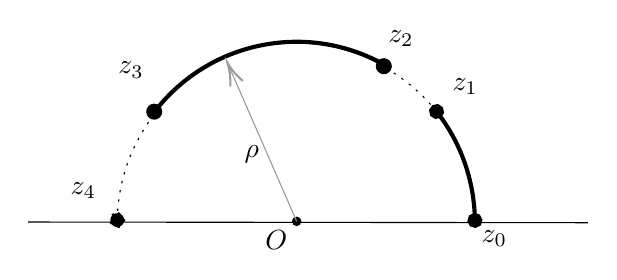
\begin{tikzpicture}[x=0.75pt,y=0.75pt,yscale=-1,xscale=1]
	%uncomment if require: \path (0,300); %set diagram left start at 0, and has height of 300
	
	%Straight Lines [id:da9415440149591279]
	\draw    (207.33,163) -- (477,163.33) ;
	%Shape: Arc [id:dp3332794895139495]
	\draw  [draw opacity=0] (268.03,109.83) .. controls (280.72,93.61) and (299.22,81.84) .. (321.1,77.99) .. controls (341.66,74.38) and (361.8,78.36) .. (378.64,87.91) -- (336.08,163.19) -- cycle ; \draw    (268.03,109.83) .. controls (280.72,93.61) and (299.22,81.84) .. (321.1,77.99) .. controls (341.66,74.38) and (361.8,78.36) .. (378.64,87.91) ; \draw [shift={(378.64,87.91)}, rotate = 25.72] [color={rgb, 255:red, 0; green, 0; blue, 0 }  ][fill={rgb, 255:red, 0; green, 0; blue, 0 }  ][line width=0.75]      (0, 0) circle [x radius= 3.35, y radius= 3.35]   ; \draw [shift={(268.03,109.83)}, rotate = 312.11] [color={rgb, 255:red, 0; green, 0; blue, 0 }  ][fill={rgb, 255:red, 0; green, 0; blue, 0 }  ][line width=0.75]      (0, 0) circle [x radius= 3.35, y radius= 3.35]   ;
	%Shape: Arc [id:dp5363284559358221]
	\draw  [draw opacity=0][line width=1.5]  (404.06,109.75) .. controls (412.6,120.61) and (418.66,133.67) .. (421.22,148.23) .. controls (422.04,152.93) and (422.47,157.61) .. (422.53,162.23) -- (336.08,163.19) -- cycle ; \draw [line width=1.5]    (404.06,109.75) .. controls (412.6,120.61) and (418.66,133.67) .. (421.22,148.23) .. controls (422.04,152.93) and (422.47,157.61) .. (422.53,162.23) ; \draw [shift={(422.53,162.23)}, rotate = 85.36] [color={rgb, 255:red, 0; green, 0; blue, 0 }  ][fill={rgb, 255:red, 0; green, 0; blue, 0 }  ][line width=1.5]      (0, 0) circle [x radius= 2.61, y radius= 2.61]   ; \draw [shift={(404.06,109.75)}, rotate = 55.82] [color={rgb, 255:red, 0; green, 0; blue, 0 }  ][fill={rgb, 255:red, 0; green, 0; blue, 0 }  ][line width=1.5]      (0, 0) circle [x radius= 2.61, y radius= 2.61]   ;
	%Shape: Circle [id:dp38847979876681604]
	\draw  [fill={rgb, 255:red, 0; green, 0; blue, 0 }  ,fill opacity=1 ] (334.67,162.67) .. controls (334.67,161.56) and (335.56,160.67) .. (336.67,160.67) .. controls (337.77,160.67) and (338.67,161.56) .. (338.67,162.67) .. controls (338.67,163.77) and (337.77,164.67) .. (336.67,164.67) .. controls (335.56,164.67) and (334.67,163.77) .. (334.67,162.67) -- cycle ;
	%Shape: Arc [id:dp030040374752331678]
	\draw  [draw opacity=0][dash pattern={on 0.84pt off 2.51pt}] (379.62,88.86) .. controls (388.96,94.22) and (397.27,101.3) .. (404.06,109.75) -- (336.65,163.92) -- cycle ; \draw [color={rgb, 255:red, 0; green, 0; blue, 0 }  ,draw opacity=1 ][dash pattern={on 0.84pt off 2.51pt}] [dash pattern={on 0.84pt off 2.51pt}]  (379.62,88.86) .. controls (388.96,94.22) and (397.27,101.3) .. (404.06,109.75) ;
	%Shape: Arc [id:dp6483332818512029]
	\draw  [draw opacity=0][line width=1.5]  (268.61,109.31) .. controls (281.31,93.08) and (299.81,81.31) .. (321.69,77.47) .. controls (342.25,73.85) and (362.38,77.83) .. (379.23,87.38) -- (336.67,162.67) -- cycle ; \draw [line width=1.5]    (268.61,109.31) .. controls (281.31,93.08) and (299.81,81.31) .. (321.69,77.47) .. controls (342.25,73.85) and (362.38,77.83) .. (379.23,87.38) ; \draw [shift={(379.23,87.38)}, rotate = 25.72] [color={rgb, 255:red, 0; green, 0; blue, 0 }  ][fill={rgb, 255:red, 0; green, 0; blue, 0 }  ][line width=1.5]      (0, 0) circle [x radius= 1.74, y radius= 1.74]   ; \draw [shift={(268.61,109.31)}, rotate = 312.11] [color={rgb, 255:red, 0; green, 0; blue, 0 }  ][fill={rgb, 255:red, 0; green, 0; blue, 0 }  ][line width=1.5]      (0, 0) circle [x radius= 1.74, y radius= 1.74]   ;
	%Straight Lines [id:da44229970288016984]
	\draw [color={rgb, 255:red, 155; green, 155; blue, 155 }  ,draw opacity=1 ]   (336.67,162.67) -- (304.13,88.17) ;
	\draw [shift={(303.33,86.33)}, rotate = 66.41] [color={rgb, 255:red, 155; green, 155; blue, 155 }  ,draw opacity=1 ][line width=0.75]    (10.93,-3.29) .. controls (6.95,-1.4) and (3.31,-0.3) .. (0,0) .. controls (3.31,0.3) and (6.95,1.4) .. (10.93,3.29)   ;
	%Shape: Arc [id:dp7257242215345958]
	\draw  [draw opacity=0][dash pattern={on 0.84pt off 2.51pt}] (250.22,162.08) .. controls (250.54,143.04) and (257.17,125.07) .. (268.38,110.6) -- (336.67,163.67) -- cycle ; \draw [color={rgb, 255:red, 0; green, 0; blue, 0 }  ,draw opacity=1 ][dash pattern={on 0.84pt off 2.51pt}] [dash pattern={on 0.84pt off 2.51pt}]  (250.22,162.08) .. controls (250.54,143.04) and (257.17,125.07) .. (268.38,110.6) ;  \draw [shift={(250.22,162.08)}, rotate = 275.14] [color={rgb, 255:red, 0; green, 0; blue, 0 }  ,draw opacity=1 ][fill={rgb, 255:red, 0; green, 0; blue, 0 }  ,fill opacity=1 ][dash pattern={on 0.84pt off 2.51pt}][line width=0.75]      (0, 0) circle [x radius= 3.35, y radius= 3.35]   ;
	
	% Text Node
	\draw (320.33,166.07) node [anchor=north west][inner sep=0.75pt]    {$O$};
	% Text Node
	\draw (310.33,124.73) node [anchor=north west][inner sep=0.75pt]    {$\rho $};
	% Text Node
	\draw (424.53,165.63) node [anchor=north west][inner sep=0.75pt]    {$z_{0}$};
	% Text Node
	\draw (410.53,92.63) node [anchor=north west][inner sep=0.75pt]    {$z_{1}$};
	% Text Node
	\draw (379.53,69.63) node [anchor=north west][inner sep=0.75pt]    {$z_{2}$};
	% Text Node
	\draw (249.53,84.63) node [anchor=north west][inner sep=0.75pt]    {$z_{3}$};
	% Text Node
	\draw (226.53,142.63) node [anchor=north west][inner sep=0.75pt]    {$z_{4}$};
	
	
\end{tikzpicture}

   }
    \caption{The curve $\G^+$ for computing the genus 1 kurtosis and its modulational dynamics. Here $z_4=\rho {\rm e}^{{\rm i}\alpha_4}=-\rho$ and $z_0=\rho {\rm e}^{{\rm i}\alpha_0}=\rho$ are fixed. When considering the modulational dynamics, $\alpha_1=\arg z_1=\arccos(q_+)$, $\alpha_3=\arg z_3=\arccos(q_-)$, where $q_-<q_+$ are given by the initial data for the Riemann problem.  At $t=0$  we have $z_2=z_1$, but for $t>0$  the motion of the point $z_2=\rho\exp\{{\rm i}\arccos(a_2(x,t))\}$ is determined through the equation \eqref{def a2 first}.}
    \label{fig:DSW-spectrum}
\end{figure} 